\documentclass[english]{presentation}
%\setbeameroption{show notes on second screen}
%\setbeameroption{show only notes}

\usepackage{chngpage}
\usepackage{array}

% Presento style file
\usepackage{config/presento}

\usepackage{textpos}
\setlength{\TPHorizModule}{1cm}
\setlength{\TPVertModule}{1cm}

\usepackage{stmaryrd}

% strikethrough text
\usepackage[normalem]{ulem}

% macros
\usepackage{mama}
\usepackage{opengames}

\addbibresource{./bibliography.bib}

\title{Games with players}
\subtitle{Towards categorical foundations of cybernetics\\[3ex]{\color{colormain}An MSP101 talk}}
\institute{University of Strathclyde}
\author{Matteo Capucci}
\date{April 29th, 2021 (Day 488 of the COVID Era)}

\begin{document}
	\begin{frame}[plain]
		\maketitle
	\end{frame}

	\begin{frame}{Intro}
	This talk gathers ideas from the last 6-24 months regarding game theory, machine learning, cybernetics, etc.

	\vfill
	\onslide<2->{Most of these are the brainchild of a whole group of people in the group -- I just packaged them together with a bow}

	\vfill
	\onslide<3->{
		Plan
		\begin{enumerate}
			\item \textbf{Game theory 101} -- concepts and terminology
			\item \textbf{Open games with players} -- from scratch
			\item \textbf{Post-credit scene}: cybernetics
		\end{enumerate}
	}
\end{frame}

	\begin{frame}{What is a game?}
	Informal definition:

	\vfill
	\begin{quotation}
		Game theory is the mathematical study of interaction among independent, self-interested agents.\\
		{\color{colornote}-- Essentials of Game Theory \cite{leyton2008essentials}}
	\end{quotation}

	\vfill
	Examples:
	\begin{enumerate}
		\item Tic-tac-toe, chess, Monopoly, etc.
		\item Economic games (includes/are included in: ecological games)
		\item Social dilemmas (PD, 'tragedy of the commons', etc.)
		\item Proof theory, model theory, etc.
		\item Machine learning
		\item \textbf{etc.}
	\end{enumerate}
\end{frame}

\begin{frame}{Representing games}
	\vfill
	\begin{enumerate}
		\item \textbf{Normal form}:
		A set of \textbf{players} $P$, an indexed set of \textbf{actions} $A : P \to \Set$, a \textbf{utility function}
		$u : \prod_{p \in P} A\; p \to (P \to R)$

		\item \textbf{Extensive form}:
		A set of \textbf{players} $P$, a \textbf{tree} representing the unfolding of the game. Nodes are assigned to players and grouped in \textbf{information sets}. Branches are called \textbf{moves}. A \textbf{utility vector} assigned to each leaf.
	\end{enumerate}

	\vfill
	\begin{center}
		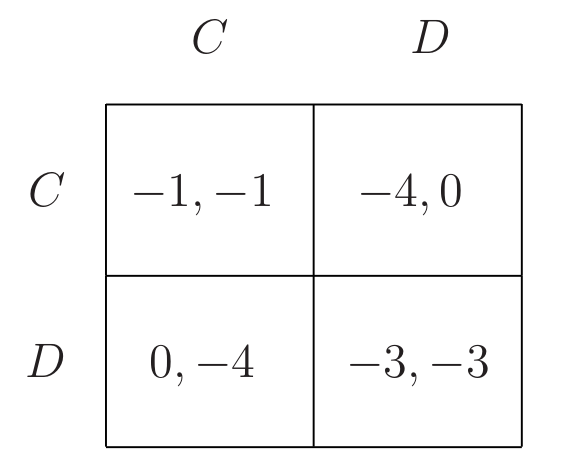
\includegraphics[width=.4\textwidth]{figures/pd_norm.png}
		\qquad
		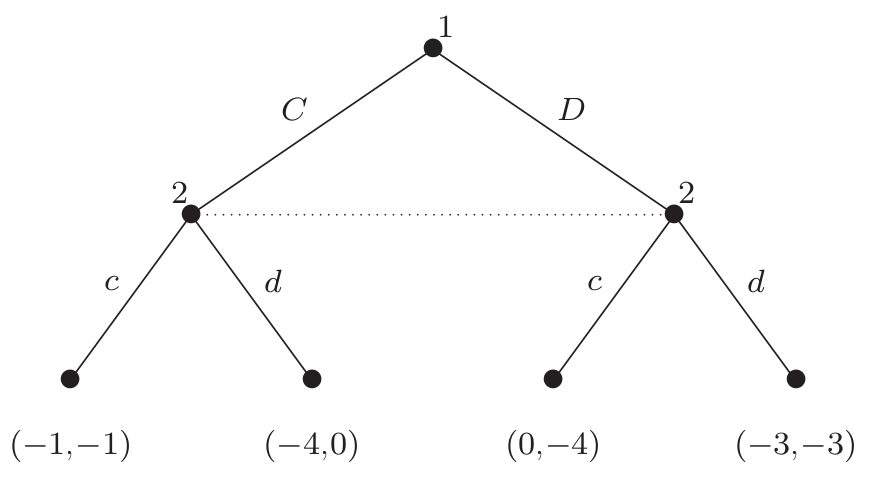
\includegraphics[width=.5\textwidth]{figures/pd_ext.png}
	\end{center}
\end{frame}

\begin{frame}{Extensive $\to$ normal}
	One can always convert an extensive form game into normal form:

	\hfill
	\begin{enumerate}
		\item Define
		\begin{equation*}
			A\; p = \sum_{x \in \text{$p$'s nodes}} \text{moves at $x$}
		\end{equation*}
		\item Define
		\begin{eqalign*}
			u(\text{action profile $a_1, \ldots, a_n$}) &=
			u(\text{path $a_1, \ldots, a_n$})\\
			&= \text{payoff at the end of the path}.
		\end{eqalign*}
	\end{enumerate}

	\vfill
	The converse is not always possible since normal-form games have too little structural information.
\end{frame}

\begin{frame}{Solving games}
	\textbf{Pre-formal definition}: A \textbf{solution concept} is a notion of `optimality' for ways to play a game.

	A 'way to play' for a player $p \in P$ is called \textbf{strategy}:
	\begin{equation*}
		\Omega\; p = \prod_{x \in \text{$p$'s nodes}} \text{moves at $x$}
	\end{equation*}
	Compare it with
	\begin{equation*}
		A\; p = \sum_{x \in \text{$p$'s nodes}} \text{moves at $x$}
	\end{equation*}

	\textbf{Key difference}: strategies are a \textbf{comprehensive plan of action}: for each \textbf{state} of the game, no matter how unlikely, we plan an \textbf{action}.

	A choice of strategy for each player is a \textbf{strategy profile}:
	\begin{equation*}
		S = \prod_{p \in P} \Omega\; p
	\end{equation*}
\end{frame}

\begin{frame}{Nash equilibrium}
	The most important (and general) solution concept is \textbf{Nash equilibrium}:

	\vfill
	\begin{definition}
		A strategy profile $s \in S$ is a Nash equilibrium if no player has interest in unilaterally deviating its strategy.
	\end{definition}

	\vfill
	e.g. for utility-maximizing players:

	\begin{equation*}
		\forall p \in P,\, \forall s'_p \in \Omega\; p \quad u_i(s[s_p/s'_p]) \leq u_p(s)
	\end{equation*}

	\vfill
	It's not the only one: SGP, ESS, $\epsilon$-Nash, trembling hand, etc.

	Afaik, all are \textbf{refinements} of Nash.
\end{frame}

\begin{frame}{Nash equilibrium: example}
	\begin{center}
		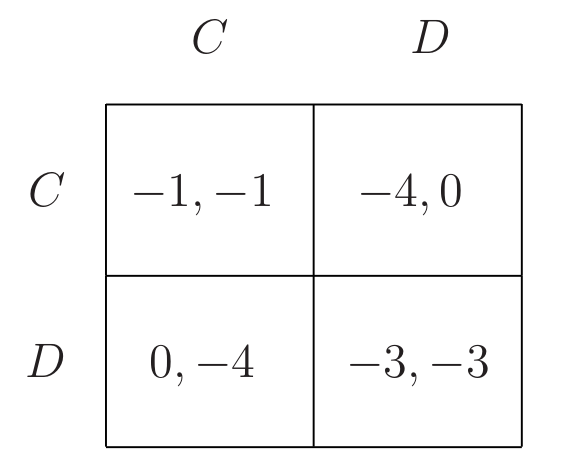
\includegraphics[width=.6\textwidth]{figures/pd_norm.png}
	\end{center}
\end{frame}

\begin{frame}{Pros and cons}
	Problems with classical game theory:
	\begin{enumerate}
		\item Games are treated \textbf{monolithically}
		\item Stuck in \textbf{early 20th century mathematical language}
		\item Denotations are quite disappointing: normal form is too opaque, extensive form is too... extended
	\end{enumerate}

	Open games are a proposed improvement:
	\begin{enumerate}
		\item Games are defined \textbf{compositionally}, including \textbf{equilibria}
		\item Mathematically more sophisticated (grounded in \textbf{category theory})
		\item Denoted by \textbf{string diagrams}: halfway between normal and extensive form
	\end{enumerate}

	It follows the ACT tradition of `opening up' systems: \emph{always consider a system as part of an environment it interacts non-trivially with}
\end{frame}

	\begin{frame}{Open games}
	\textbf{Warning}: Open games are compositional structures, hence the single building blocks do not make much sense from a classical standpoint -- you have to put them together to get something meaningful

	\vfill
	Informally: an 'atomic' open game is a forest of bushes
	(pic)
\end{frame}

\begin{frame}{Open games}
	First of all, let's model the information flow of a game.
	(pic of a tree)
	There's two phases in a game
	\begin{enumerate}
		\item The 'play' or 'forward phase': players takes turn and make their own decisions until a leaf is reached
		\item The 'coplay' or 'backward phase': payoffs propagate back to player along the tree
	\end{enumerate}

	The backward phase is done for analysis purposes: we observe how different decisions would bring about different payoffs (\textbf{backward induction})
\end{frame}

\begin{frame}{Open games}
	A \textbf{lens} models exactly this bidirectional information flow:

	(pic of a lens)

	Slogan: `\textbf{Time flows clockwise}'

	\begin{definition}
		Let $\cat C$ be a cartesian category (think: sets \& functions). A \textbf{lens} $(X,S) \to (Y,R)$ is a pair of maps
		\begin{eqalign*}
			\mathsf{view} &: X \to Y\\
			\mathsf{update} &: X \times R \to S
		\end{eqalign*}
	\end{definition}

	Intuition: \textbf{view} corresponds to the forward step, \textbf{update} to the backward step.
\end{frame}

\begin{frame}{Open games}
	So a game can be represented naively as a lens $(X,S) \to (Y,R)$ where
	\begin{description}
		\item[...] $X$ are \textbf{states of the game}
		\item[...] $Y$ are \textbf{moves}
		\item[...] $R$ are \textbf{utilities}
		\item[...] $S$ are \textbf{coutilities}
	\end{description}

	In open games we call the forward part of a lens '\textbf{play}' and backward part '\textbf{coplay}'
\end{frame}

\begin{frame}{Open games}
	What's coutility?

	\begin{quotation}
		For a given node $x$ in a game, a player’s continuation value (also called continuation payoff) is the payoff that this player will eventually get contingent on the path of play passing through node $x$.\\
		{\color{colornote}-- Strategy \cite{strategy}}
	\end{quotation}

	The coplay function takes on this job. In classical game theory it's hidden in backward induction.
	It doesn't \textbf{have to} be trivial, but it often is.
\end{frame}

\begin{frame}{Open games}
	Lenses, hence games, can then be composed in at least two ways:

	(sequential)

	(parallel)
\end{frame}

\begin{frame}{Open games}
	We can use sequential composition to give a lens a \textbf{context}, i.e. an initial \textbf{state} and a \textbf{payoff function}

	(pic)

	Remember: '\textbf{time flows clockwise}'
\end{frame}

\begin{frame}{Open games}
	What's missing?

	\begin{quotation}
		What does it mean to say that agents are self-interested? [...] [I]t means that each agent has \textbf{[their] own description} of which \textbf{states of the world [they like]}—which can include good things happening to other agents—and that \textbf{[they act]} in an attempt to bring about these states of the world.\\
		{\color{colornote}-- Essentials of Game Theory \cite{eogt}}
	\end{quotation}

	Three things:
	\begin{enumerate}
		\item A way for agents to \textbf{act in the world}
		\item A way for agents to \textbf{represent the world}
		\item A way for agents to \textbf{evaluate the world}
	\end{enumerate}

	At the moment, agents do not intervene in the unfolding of the game: plays and coplays are fixed

	We need to give a 'steering wheel' to agents
\end{frame}

\begin{frame}{Interlude I: the Para construction}

	Para originates in \cite{backpropasafunctor} an has been adopted by this group (Bruno) to represent all sort of stuff. Also Toby Smithe has come up with a Para-like construction, Proxy.
\end{frame}

\begin{frame}{Interlude I: the Para construction}
	\begin{definition}
		When $\cat C$ is symmetric monoidal, $\Para(\cat C)$ is the category of parametrized morphisms of $\cat C$:
		\begin{enumerate}
			\item objects are the same,
			\item a morphism $A \to B$ is given by a choice of parameter $P : \cat C$ and a choice of morphism $P \otimes A \to B$ in $\cat C$:
		\end{enumerate}
	\end{definition}

	(pic of para morphism)
\end{frame}


\begin{frame}{Interlude I: the Para construction}
	$\Para(C)$ is again symmetric monoidal:

	(pic of seq comp)

	(pic of par comp)

	and, most importantly, it's a \textbf{bicategory}

	(pic of 2-cell)
\end{frame}

\begin{frame}{Interlude I: the Para construction}
	Now, if our morphisms are `bidirectional', we get an even more interesting picture:

	(pic of para optic)

	If we peek inside, we can see the new information flow:

	(pic of para lens, opened up)
\end{frame}

\begin{frame}{Open games}
	\textbf{Idea}: if 'games without agency' are lenses, 'games with agency' are \emph{parametrized} lenses:

	\begin{itemize}
		\item parameters are \textbf{strategies}: \textbf{the ways an agent acts} in the world
		\item coparameters are \textbf{'costrategies'}: \textbf{the ways an agent represents} the world
	\end{itemize}

	The only piece still missing is ways for agents to \textbf{evaluate} the world.
\end{frame}

\begin{frame}{Interlude II: selection functions}
	\begin{definition}
		A \textbf{continuation} on a object $X$ with scalars an object $R$ is a map
		\begin{equation*}
			K_R(X) = (X \to R) \to R
		\end{equation*}
	\end{definition}

	It's a `generalized quantifier': $\max$, $\min$, $\exists$, $\forall$

	If the ambient category is cartesian closed, $K_R$ defines a monad.
\end{frame}

\begin{frame}{Interlude II: selection functions}
	Selection functions `realize' quantifiers:

	\begin{definition}
		Def. A \textbf{selection function} on a object X with scalars an object R is a map
		\begin{equation*}
			J_R(X) = (X \to R) \to X
		\end{equation*}
	\end{definition}

	Examples: $\argmax$, $\argmin$, Hilbert's $\varepsilon$

	If the ambient category is cartesian closed, $J_R$ defines a monad.
\end{frame}

\begin{frame}{Interlude II: selection functions}
	Notice: often quantifiers are realized by multiple elements...

	(ambiguous max function)

	So a better type for selection functions is

	\begin{equation*}
		(X \to R) \to \copow X
	\end{equation*}

	where $\copow$ is the powerset monad.
\end{frame}

\begin{frame}{Interlude II: selection functions}

	Also notice:

	\begin{diagram*}
		(X \to R) \arrow{r} \& \copow  X\\[-8ex]
		\text{costate of $(X, R)$} \& \text{state of $(X, R)$}
	\end{diagram*}

	so we arrive to a general definition:

	\begin{definition}
		Let $\cat C$ be a monoidal category. Then the selection functions functor is
		given by
		\begin{eqalign*}
			\Sel : \cat C &\longto \Cat\\
			X &\longmapsto \cat C(X, I) \to \copow \cat C(I,X)
		\end{eqalign*}
	\end{definition}

	The codomain is $\Cat$ since this set is ordered by pointwise inclusion:
	\vspace{-2ex}
	\begin{equation*}
		\varepsilon \leq \varepsilon' \sse \forall k \in \cat C(X,I),\ \varepsilon(k) \subseteq \varepsilon'(k)
	\end{equation*}
\end{frame}

\begin{frame}{Interlude II: selection functions}
	$\Sel$ is a functor because it also acts on morphism by \textbf{pushforward}:

	(pic from wiki)

	\textbf{Idea}: selection functions are a relation between states and costates
	(Probably better: selection functions are predicates on \emph{contexts})
\end{frame}

\begin{frame}{Interlude II: selection functions}
	Finally, $\Sel$ is \textbf{lax monoidal} with \textbf{Nash product}:

	\begin{eqalign*}
		\boxtimes &: \Sel(X) \times \Sel(Y) \to \Sel(X \otimes Y)\\
		&(\varepsilon \boxtimes \eta)(k) = \{ x \otimes y \in (X \otimes y)_* \varepsilon(k) \cap (x \otimes Y)_* \eta(k) \}
	\end{eqalign*}

	(pic)
\end{frame}

\begin{frame}{Open games}
	To see why we call this the Nash product, let's go back to games...

	(pic of para optic)

	At this point, we only miss one piece of data:
	\begin{enumerate}
		\item[3] A way for agents to \textbf{evaluate the world}
	\end{enumerate}

	\vfill
	Idea: for each player, we pick a selection function
	\begin{equation*}
		\varepsilon \in \Sel(\Omega, \Comega)
	\end{equation*}
	to model their preferences
\end{frame}

\begin{frame}{Open games}
	Now, careful. Recall:

	\vfill
	\begin{quotation}
		Game theory is the mathematical study of \textbf{interaction} among independent, self-interested \textbf{agents}.\\
		{\color{colornote}-- Essentials of Game Theory \cite{eogt}}
	\end{quotation}


	A game factors in two parts
	\begin{enumerate}
		\item An \textbf{arena}, which models the {interaction patterns} in the game
		\item A set of \textbf{agents}, i.e. the players, which make \textbf{decisions} at different points of a game
	\end{enumerate}

	Without (2) a game would be only a \textbf{dynamical system}, whose dynamic is fixed.
	Instead, in a game \textbf{agents can vary the dynamics in response to the observed unfolding of the interaction}.
\end{frame}

\begin{frame}{Open games}
	Therefore: \textbf{agents live in the parametrization direction}

	(pic: para optic with arena and agents areas highlighted)

	The arena plays the role of a costate to them:

	(pic of $\top$ action)
\end{frame}

\begin{frame}{Open games}
	Finally, if arenas can be defined '\textbf{locally}' because they are information plumbing, agents' interests can't since they are defined '\textbf{globally}': an agent might observe and interact with the arena at multiple, causally 'far' points.

	We take advantage of the 2-cells in Para(Lens) to handle this:

	(pic)
\end{frame}

\begin{frame}{Open games}
	Great! So an open game is

	\begin{definition}
		\begin{enumerate}
			\item A \textbf{parametrized lens}
			\begin{equation*}
				\G : (X, S) \nlongto{(P, P')} (Y,R)
			\end{equation*}
			\item A set of players $\{1, ..., n\}$, each represented by their own \textbf{selection function}
			\begin{equation*}
				\varepsilon_i \in \Sel(\Omega_i, \Comega_i)
			\end{equation*}
			\item A \textbf{wiring 2-cell}:
			\begin{equation*}
				w : \prod_{i \in I} (\Omega_i, \Comega_i) \longto (P,P')
			\end{equation*}
		\end{enumerate}
	\end{definition}
\end{frame}

\begin{frame}{Open games}
	Equilibria are given by

	\begin{equation*}
		\eq(x,u) = (\varepsilon_1 \boxtimes \cdots \boxtimes \varepsilon_n)(w ; (x ; G ; u)^\top)
	\end{equation*}

	It can be shown that this definition is compositional in the natural way, and recovers Nash equilibria as a solution concept (which justifies calling $\boxtimes$ \textbf{Nash product})
\end{frame}

\begin{frame}{Open games}
	This solves long-standing problems with open games:

	\begin{enumerate}
		\item We finally compute ther \textbf{right set of Nash equilibria}
		\item We can handle situations of \textbf{imperfect recall}
		\item We can define equilibria for \textbf{internal choice}
		\item We can even model coalitional games (future work)
	\end{enumerate}

	Still a lot to explore.
\end{frame}

	\begin{frame}{Cybernetics}
	From $\kappa\upsilon\beta\varepsilon\rho\nu\alpha\omega$ (\emph{to govern, to steer}):
	\vfill

	\begin{quotation}
		Science concerned with the study of systems of any nature which are capable of receiving, storing and processing information so as to use it for control.
		{\color{colornote}-- Kolmogorov}
	\end{quotation}

	Lenses model dynamical systems (see: \cite{myers2020double})\\
	\textbf{\color{coloraccent}Parametrized lenses (+ decorations) model cybernetic systems!}

	\vfill
	The missing bits are \textbf{storage} and \textbf{feedback}.

	\vfill
	{\color{colornote}
	$\underbrace{\text{Parametrized $\cdots$ parametrized}}_{\text{$n$ times}}$ lenses model \textbf{...?}\\[1.5ex]
		\hspace{5ex} \textbf{Hierarchical agency?}
	}
\end{frame}

\begin{frame}{Higher-order cybernetics}
	Agents
	\begin{enumerate}
		\item act in the arena,
		\item then \textbf<2->{observe} the result of their behaviour,
		\item then change their action accordingly,
	\end{enumerate}
	until an equilibrium is reached.

	\onslide<2->{
	\vfill
	\begin{tabular}{p{.2\textwidth}|p{.12\textwidth}p{.12\textwidth}p{.12\textwidth}p{.1\textwidth}}
		& \textbf{1st} & \textbf{2nd} & \textbf{3rd} & $\cdots$\\
		\hline
		non-trivial\newline observation     &     & yes & yes & $\cdots$\\[2ex]
		\hline
		non-trivial analysis                &     &     & yes & $\cdots$\\[2ex]
		\hline
		$\qquad \vdots$                     &     &     &     & $\ddots$
	\end{tabular}
	}
\end{frame}

\begin{frame}{Periodic table of cybernetic types}
	\vspace{-2ex}
	Reasoning negatively:
	\vspace{2ex}

	\vfill
	\begin{tabular}{p{.16\textwidth}|p{.1\textwidth}p{.1\textwidth}p{.1\textwidth}p{.1\textwidth}p{.1\textwidth}p{.01\textwidth}}
		% static - closed dynamical - open dynamical - cybernetic - 2nd-order cybernetic - ...
		& \textbf{-2nd} & \textbf{-1st} & \textbf{0th} & \textbf{1st} & \textbf{2nd} & $\cdots$\\
		\hline
		{\color{coloraccent}non-trivial system}      &     & yes & yes & yes & yes & $\cdots$\\[2ex]
		\hline
		{\color{coloraccent}non-trivial context}     &     &     & yes & yes & yes & $\cdots$\\[2ex]
		\hline
		{\color{coloraccent}non-trivial interaction} &     &     &     & yes & yes & $\cdots$\\[2ex]
		\hline
		non-trivial observation                      &     &     &     &     & yes & $\cdots$\\[2ex]
		\hline
		$\qquad \vdots$                              &     &     &     &     &     & $\ddots$
	\end{tabular}
\end{frame}

\begin{frame}{Games vs. learners}
	\begin{center}
		\includegraphics[clip, page=16, trim=2cm 5cm 5cm 2cm, width=.8\textwidth]{figures/drawings.pdf}
	\end{center}

	\vfill
	A learner produces its own selection function as a fixpoint:

	\begin{equation*}
		p \in \eq(x,u) \sse p = p \cmp GD \cmp w \cmp (x \cmp \L \cmp u)^\top
	\end{equation*}
\end{frame}

\begin{frame}{2nd order cybernetics}
	Given a parameter $p \in P$, a learner can only observe $\L^\top$ on an infinitesimal neighbourhood of $p$\\
	\qquad $\rightsquigarrow$ \textbf{2nd-order cybernetic systems}

	\vfill
	We can consider $\Para(\Lens(\cat{Smooth}))$ a \textbf{2nd-order \emph{cybernetic doctrine}} (terminology borrowed from \cite{myers2021cst})

	\vfill
	This is actually a strength:
	\begin{enumerate}
		\item We can encode the selection in the parameter dynamics
		\item We can analyze locally and iteratively\\(vs. games `global and one-step')
	\end{enumerate}
\end{frame}


	\begin{framecard}
		{\color{white}
		\bfseries

		\hugetext{Thanks for your attention!}
		\largetext {Questions?}}
	\end{framecard}

	\begin{frame}{References}
		\nocite{*}
		\printbibliography
	\end{frame}
\end{document}
